%%!TEX root = diss.tex

\chapter{Collisional Langevin model of bedload sediment velocity distributions}
\label{ch:langevin}
\section{Introduction}

Bed load transport rates show wide and frequent fluctuations which originate from coupling between the fluid and granular phases.
Owing to these fluctuations, measured transport rates often show slow convergence through time \citep{Dhont2018,Turowski2010}, and predicted rates can deviate from measured values by several orders of magnitude \citep{Recking2012,Martin2003}.
These challenges limit numerous ecological and engineering applications that rely on sediment transport predictions \citep{Gaeuman2017,Malmon2005}.
In recent decades, stochastic formulations of the bed load flux have become increasingly popular for their potential to predict the mean transport rates required by applications while also predicting the magnitude of transport fluctuations and quantifying the dependence of measurements on the observation scale (secs. \ref{sec:birthdeath}-\ref{sec:renewal}).
Recent indications that sediment transport fluctuations might explain longstanding open problems in alluvial channel stability, such as channel width maintenance \citep{Abramian2019,Abramian2020} and bedform initiation \citep{Jerolmack2005,Bohorquez2016} provide additional motivation to develop these stochastic approaches.
One subset of stochastic methods expresses downstream transport rates as a sum over the instantaneous streamwise velocities of all particles in motion within a control volume (sec. \ref{sec:birthdeath}).
This formulation requires the instantaneous velocity distributions of sediment particles \citep{Lajeunesse2010}, although understanding of these distributions remains limited.
There is as of yet no consensus on the shape of the bedload velocity distribution, and although the models described in section \ref{sec:langevin} of the introduction have described some extreme end-member distributions \citep[e.g.][]{Fan2014,Ancey2014}, no models have been developed that describe the full range of experimental observations \citep{Lajeunesse2010,Fathel2015,Heyman2016,Liu2019,Houssais2012}.
In this chapter, I develop a stochastic model of particle velocities which addresses this shortcoming.

High-speed video experiments have measured different streamwise particle velocity distributions without indicating why one distribution or another appears in a given set of hydraulic and sedimentary conditions.
One set of studies has shown exponential particle velocity distributions \citep{Charru2004,Lajeunesse2010,Roseberry2012,Seizilles2014,Fathel2015,Fathel2016}.
These experiments involve uniformly-sized small sands or glass beads ($~0.05-2$mm) in turbulent and subcritical flows, but not always; the experiments of \citet{Lajeunesse2010} were supercritical, while the experiments of \citet{Charru2004} and \citet{Seizilles2014} were viscous.
A second set of studies have shown Gaussian particle velocity distributions \citep{Ancey2014,Heyman2016,Martin2012}. In these experiments, particles are typically larger ($2-8$mm) uniformly-sized gravels or glass beads, and flows are generally turbulent and super-critical.
Other experiments display velocity distributions that are intermediate between exponential and Gaussian extremes that appear visually more like a Gamma distribution \citep{Houssais2012, Liu2019}.
The \citet{Houssais2012} experiments involved a binomal distribution of glass beads with diameters $0.7$mm and $2.2$mm in turbulent and supercritical flow conditions, while the \citet{Liu2019} experiments used sand having median diameter $1.1$mm. Flows were again turbulent and subcritical.
From this experimental record, the velocity distribution shape apparently does not consistently relate to super or sub-critical flow conditions, whether sediment grains are natural (sand, gravel) or synthetic (glass beads), or whether the flow is laminar or turbulent.
However there is a loose trend within the particle size. Smaller particles tend to show more exponential-like distributions \citep[e.g.][]{Fathel2015}, while larger ones show Gaussian distributions \citep[e.g.][]{Heyman2016}. This summary suggests that the shape of streamwise bed load velocity distribution could be controlled by the particle size.

Existing models of streamwise bed load velocities can be divided into computational and stochastic physics categories.
Computational models numerically integrate some approximate coupled dynamics for individual grains and the fluid, generally modelling particles as spheres interacting through repulsive forces, and the flow using direct simulation of the Navier-Stokes equations or some related approximation (such as large eddy simulation or the St-Venant equations).
When streamwise particle velocities have been analyzed in such simulations, they show exponential tails \citep{Gonzalez2017,Furbish2013} that agree with one subset of the experimental data.

Several stochastic models have incorporated fluctuating driving and resisting terms into the Newtonian dynamics of individual grains to develop Langevin-like descriptions of bed load particle motions (sec. \ref{sec:langevin}). \citet{Fan2014} represented turbulent drag as Gaussian white noise and included a static Coulomb friction term to model particle-bed collisions, while \citet{Ancey2014} applied an Ornstein-Uhlenbeck process which combines the fluid and driving forces were lumped into a velocity-dependent force, while Gaussian white noise represents fluctuations.
Each of these models derives one end-member distribution from among the range of distributions reported in experiments.
A physical description for the full range of experimentally-observed bedload velocity distributions remains an elusive target.

In this chapter I explore the possibility that the shape of the particle velocity distribution is controlled by momentum dissipation during particle-bed collisions.
In the theory of granular gases, dissipative collisions are known to cause departures toward an exponential velocity distribution from the ideal Gaussian form expected from perfectly elastic collisions \citep{Brilliantov2004}.
Gas theory formulates particle-particle collisions as a nonlocal integral within the master equation for the probability distribution of particle velocity called the Boltzmann equation \citep{Landau1969,Chapman1970}.
Collisions in these models involve episodic kicks to the particle momenta at random times, parameterized by billiard ball-like models of the underlying rigid body dynamics \citep[e.g.][]{Brach1989}.
In contrast, current stochastic models of bedload transport appear highly simplified, treating collisions instead with static Coulomb or velocity-dependent drag.

Taking inspiration from granular gas theory, I develop in this chapter an improved model for sediment grains in transport, including episodic particle-bed collisions.
The driving motivation is to test the hypothesis that particle-bed collision characteristics can explain the range of experimentally-observed streamwise bed load particle velocity distributions.
A secondary one is to introduce more realistic forces into earlier stochastic descriptions of individual bed load particle dynamics. 
I develop the model and explain its key assumptions in section \ref{sec:langmodel}. Then I present the analytical solution of the model and other major results in \ref{sec:langresults}. Finally I discuss the implications of these results, summarize key findings, and suggest ideas for further research in sections \ref{sec:langdiscussion} and \ref{sec:langconclusion}.


\section{Mechanistic description of particle velocities}
\label{sec:langmodel}

Figure \ref{fig:fig1} indicates the configuration of the model in this chapter.
Nearly spherical cohesionless particles of diameter $d$ and mass $m$ move as bed load down a slope inclined at an angle $\theta$ in a steady turbulent shear flow.
The flow is just strong enough to drive grains into the rarefied transport typical in gravel-bed rivers: particles saltate downstream through a sequence of particle-bed collisions. 
Moving particles collide often with stationary particles, but rarely with other moving particles.

Particles respond to turbulent drag forces $F_D(t)$ and episodic particle-bed collision forces. In contrast to the computational physics approach, I do not aim to characterize the exact timeseries of the forces on an individual particle. Instead, I model the ensemble of possible force timeseries that particles could conceivably experience. Each possibility implies a different possible velocity timeseries $u(t)$ in the downstream direction.
The objective is to calculate the probability distribution $P(u)$ of this downstream velocity by averaging over the ensemble of forces.
I include the most realistic article-bed collision and fluid forces possible while still allowing for analytical solutions. 

\subsection{Episodic collisions}
Collisions between bedload particles dissipate momentum, partly by converting it to vertical, lateral, or rotational momentum, partly by deforming particles and generating heat \citep{Schmeeckle2014,Williams2021}, and partly by pressurizing the fluid \citep{Joseph2001,Schmeeckle2001}. 
The microscopic details of particle-particle collisions have been thoroughly studied \citep{Brach1989, Lorenz1997,Montaine2011}. Here, we introduce a simple elasticity parameter $\varepsilon$ as a first attempt at the problem, as indicated in figure \ref{fig:fig1}. This elasticity characterizes the fraction of downstream momentum lost in a collision. If the streamwise velocity just prior to a collision is $u$, just after the collision it becomes $\varepsilon u$. The elasticity ranges from $\varepsilon=0$, representing a completely inelastic collision, to $\varepsilon=1$, representing a completely elastic collision.
\begin{figure}
	\centerline{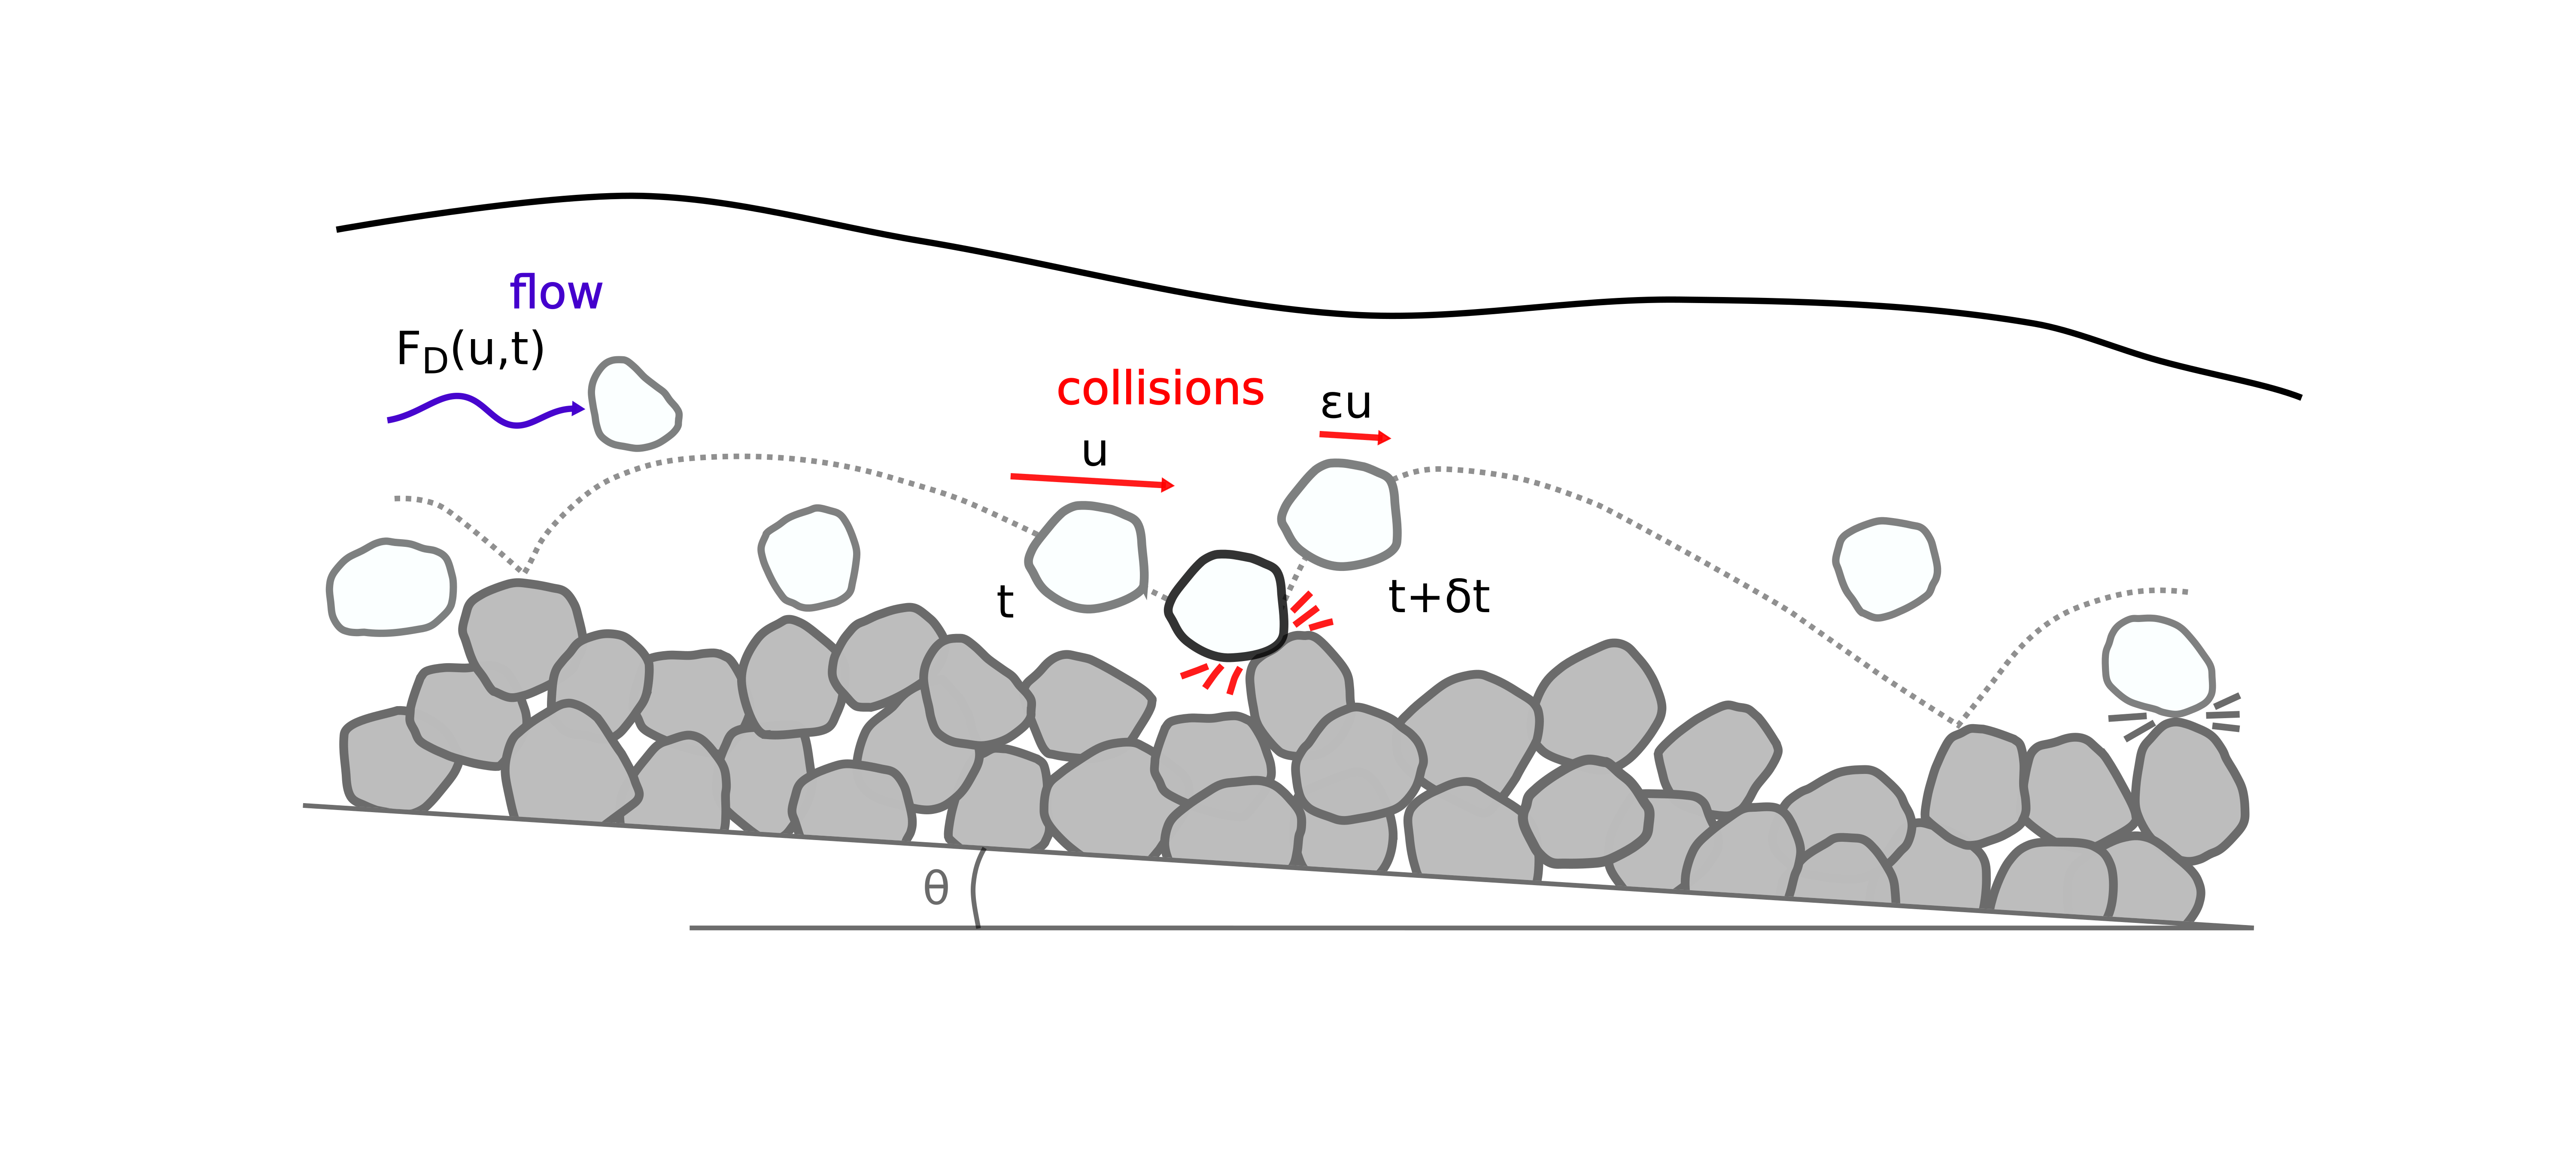
\includegraphics{./figures/ch5/Fig1Concept.png}}
	\caption{Definition sketch of rarefied sediment transport with turbulent fluid drag and particle-bed collision forces. During saltation, pre-collisional streamwise velocities $u$ are transformed to postcollisional velocities $\ve u < u$.}
	\label{fig:fig1}
\end{figure}

Since the elasticity combines effects of particle shape and collision geometry and should vary from one collision to the next, the elasticity $\varepsilon$ is interpreted as a random variable, characterized by a statistical distribution $\rho(\varepsilon)$.
Some granular gas models have also included random elasticity \citep[e.g.][]{Serero2015}.

Assuming that the number of collisions per unit time is $\nu$ and that the time intervals between subsequent particle-bed collisions are exponentially distributed \citep{Gordon1972}, the collision force in the downstream direction can be written as a Poisson pulse noise (sec. \ref{sec:einflux}):
\be F_C(u,t) = - m u \sum_{k=1}^{N_\nu(t)}(1-\varepsilon_k)\delta(t-\tau_k). \label{eq:col} \ee
Here, $N_\nu(t)$ is the number of collisions in time $t$ (a Poisson random variable), the $\tau_k$ ($k=1,2,\dots$) are times at which collisions occur, and the $\varepsilon_k$ are the elasticity coefficients, drawn from the distribution $\rho(\varepsilon)$ characterizing the fraction of momentum lost in each particle-bed collision.
This collision force is a sequence of random impulses which are proportional to the pre-collisional streamwise momentum. This collision model should be adequate when the contact times between moving and resting particles are small compared to the times between collisions. These conditions are always satisfied for the idealized saltation trajectories depicted in figure \ref{fig:fig1}.

\subsection{Turbulent fluid forces}
Fluid forces on a coarse particle in a viscous flow depend on the Reynolds number $\Re_p = d V/\nu$ defined by the particle size $d$, slip velocity $V$ between particle and fluid, and kinematic viscosity $\nu$.
These forces have been calculated analytically from the Navier-Stokes equations for vanishing $\Re_p$ and include acceleration, history, and velocity-dependent drag terms \citep{Hjelmfelt1966, Maxey1983, Auton1987}.
At realistic $\Re_p$, analytical results are inaccessible, so it is standard to include empirical corrections to the small $\Re_p$ formulas \citep{Schmeeckle2007,Clift1978}.
A dominant contribution to the downstream drag force $F_D$ on nearly spherical particles at large $\Re_p$ can be written $F_D = \frac{\pi}{8}
\rho_f d^2 C_D(\Re_p) |V|V$, where $\rho_f$ is the fluid density, $d$ is the particle diameter, $C_D(\Re_p)$ is an empirical drag coefficient, and $V = U-u$ is the slip velocity between the fluid ($U$) and particle ($u$) velocities \citep{Coleman1967, Schmeeckle2007, Dwivedi2012}.
In this study, I leave out acceleration and history terms for analytical tractability, although they are certainly relevant in coarse sediment transport \citep{Michaelides1997,Armenio2001}.

Drag forces have been argued to fluctuate rapidly compared to the inertial response times of submerged grains \citep{Fan2014}, and the magnitude of drag fluctuations has been observed to follow a Gaussian distribution \citep{Hofland2006,Schmeeckle2007,Dwivedi2010,Celik2014}.
These ideas allow two major simplifications of the above drag force.
First, the drag can be split into quasi-steady and fluctuating components \citep{Michaelides1997}, and second, drag fluctuations can be modelled a Gaussian white noise, where the fluctuations are symmetric, the autocorrelation time is negligible, and the strength of fluctuations is described by a diffusivity $D$ \citep{Fan2014,Ancey2014}. 
Defining $\bar{V}$ as a representative slip velocity to be specified more carefully later,  $\bar{C}_D$ as the empirical drag coefficient evaluated at this slip velocity, and $\xi(t)$ as a Gaussian white noise of mean $0$ and variance $1$ \citep{Gardiner1983}, the fluid drag can be written
\be F_D(t) = \Gamma + \sqrt{2 D } \eta(t), \label{eq:drag}\ee
where $\Gamma = \frac{\pi}{8}
\rho_f d^2 \bar{C}_D \bar{V}^2$ is the steady component of the drag.

\subsection{Langevin equation for collisional bedload transport}

With the above forces, the Langevin equation $m\dot{u}(t) = F_D(t) + F_C(t)$ for the sediment dynamics becomes
\be m \dot{u}(t) = \Gamma + \sqrt{2D}\eta(t) - m u(t) \xi_{\nu, \ve}(t). \label{eq:langevin} \ee
This equation replaces the steady friction terms of earlier models with an episodic term, designed to provide a more realistic representation of particle-bed collisions.
Mathematically, equation \ref{eq:langevin} is a Langevin-like equation representing a jump-diffusion process \citep{Daly2006} with multiplicative Poisson noise \citep{Dubkov2016,Denisov2009}. 
Collisions introduce ``jumps" in velocity while turbulent generates "diffusion". The collision term is "multiplicative" in the sense that $u$ multiplies the Poisson noise.

Equations like \ref{eq:langevin} have long been studied in the stochastic physics literature \citep{Hanggi1978,VanDenBroeck1983}, but solving such equations remains extremely challenging \citep{Daly2010,Mau2014,Dubkov2019}.
One issue is that multiplicative white noises imply the prescription dilemma of stochastic calculus \citep{Risken1989,Gardiner1983}, meaning \ref{eq:langevin} is not defined without further specifying an integration rule \citep{Suweis2011}.
Here, the Ito interpretation (lower endpoint integration rule) is the physical choice the energy dissipated by collisions depends strictly on pre-collisional velocities, not post-collisional \citep[e.g.][]{Gardiner1983} since.
Given this integration rule, the remaining issues are to obtain the master equation characterizing the ensemble of velocities defined by \ref{eq:langevin}, and then to solve this equation for the velocity distribution $P(u)$.

\subsection{Chapman-Komogorov equation and particle-bed collision integral}

The equation governing the streamwise velocity distribution $P(u,t)$ is derived in appendix section \ref{sec:langmasterderiv} with a limiting procedure, providing
\be \nu^{-1}\partial_t P(u,t) = - \tilde{\Gamma} \partial_u P(u,t) + \tilde{D} \partial_u^2 P(u,t) + I_c(u,t). \label{eq:master} \ee
In this equation, I introduced the scaled parameters $\tilde{\Gamma} = \Gamma/(\nu m)$ and $\tilde{D} = D/(\nu m)$ that scale the steady and fluctuating components of the fluid force against the collision rate $\nu$. The term
\be \mathcal{I}_c(u,t) = - P(u,t) + \int_0^1 \frac{d\ve}{\ve}P\big(\frac{u}{\ve},t \big) \rho(\ve) \label{eq:colint} \ee
is a ``collision integral" term representing particle-bed collisions.

Equation \ref{eq:master} is a nonlocal extension of the Fokker-Planck equation used in earlier bed load models \citep{Fan2014,Ancey2014}. 
Nonlocality is introduced by the collision integral \ref{eq:colint} which transfers probability from higher pre-collisional velocities $u/\varepsilon$ to lower post-collisional velocities $u$.
This term is analogous to the collision integral within the Boltzmann equation of kinetic theory \citep{Duderstadt1979, Brilliantov2004}. Physically, it corresponds to binary collisions between particles having different masses and random resitution coefficients \cite{Serero2015} in the limit that the mass of one particle (here, the particle resting on the bed) diverges to infinity.
Mathematically, the collision integral represents the probability distribution of the product between the elasticity $\varepsilon$ and the downstream momentum $m u$ \citep[c.f.][]{Feller1968}.


Owing to its nonlocality, equation \ref{eq:master} does not admit analytical solutions as is, so further approximation is necessary.
Assuming the distribution of elasticity $\rho(\varepsilon)$ is sharply peaked at some most common (mode) value $\varepsilon'$, which is the case in experiments of rigid body collisions \citep{Glielmo2014}, allows for a Kramers-Moyal type expansion of the particle-bed collision integral \citep{Gardiner1983}.
Expanding all terms in the integrand except $\rho(\varepsilon)$ provides
\be \mathcal{I}_c(u,t) = -P(u,t) + \frac{1}{\varepsilon'}P\big(\frac{u}{\ve'},t \big) + \sum_{k=1}^\infty \frac{\alpha_k }{k!}(\ve - \ve')^k \Big[\frac{1}{\ve}P\big(\frac{u}{\ve}\big)\Big]^{(k)}\Big|_{\ve=\ve'},\label{eq:expansion}\ee
where the $\alpha_k = \int_0^1 d\ve \rho(\ve) (\ve-\ve')^k $ are the central moments of $\ve$ around the mode elasticity $\ve'$ and the superscript $(k)$ denotes the $k$th derivative.

In what follows, I drop all but the first two terms in this expansion to obtain the leading order contribution of particle-bed collisions to the velocity distribution.
Higher orders could always be included later by perturbation theory \citep{Morse1953}.
I solve the resulting approximate equation in steady-state, when $\partial P(u,t)/\partial t = 0$. Equation \ref{eq:master} indicates that this solution will be a good approximation to the time-dependent problem when particle motions generally survive multiple collisions ($t\gg \nu^{-1}$).

\section{Results}
\label{sec:langresults}

\subsection{Derivation of the bedload velocity distribution}
\label{sec:langsolution}
Hereafter I drop the prime on the most common streamwise restitution coefficient $\ve'$.
With the truncation to two terms, equation \ref{eq:master} gives 
\be 0 = -\tilde{\Gamma}\partial_u P(u) + \tilde{D}\partial_u^2 P(u) -P(u) + \frac{1}{\ve} P\big(\frac{u}{\ve}\big),\label{eq:governer} \ee
which is an advanced functional differential equation. This equation is ``functional" in the sense that it is nonlocal in velocity due to the last term on the right hand side, and it is ``advanced" in that $u/\ve$ is advanced beyond the argument $u$ involved in the rest of this equation (since $0<\ve<1$).
Such equations seen some attention in the mathematics literature, where they are sometimes called pantograph equations \citep{Hall1989, Kim1998,Zaidi2015}.

In the appendix section \ref{sec:langsteadyderiv} I solve equation \ref{eq:governer} using Laplace transforms, providing
\begin{multline} P(u) = \frac{\theta(-u)}{K_+}\sum_{l=0}^\infty \frac{\ve^{-l}e^{\lambda_+\ve^{-l}u}}{\prod_{m=1}^l(-\tilde{D} \lambda_+^2 \ve^{-2m} + \tilde{\Gamma} \lambda_+ \ve^{-m} + 1) } 
	\\+ \frac{\theta(u)}{K_-}\sum_{l=0}^\infty \frac{\ve^{-l}e^{\lambda_-\ve^{-l}u}}{\prod_{m=1}^l(- \tilde{D} \lambda_-^2 \ve^{-2m} + \tilde{\Gamma} \lambda_- \ve^{-m} + 1) } \label{eq:steadystate}. \end{multline}
The factors $\lambda_\pm$ are defined in appendix equations \ref{eq:lambdas}. They are proportional to $\tilde{\Gamma}/\tilde{D}$. 
The normalization factors are $K_\pm$ are 
\be K_\pm = \tilde{D}(\lambda_+-\lambda_-)\prod_{l=1}^\infty (- \tilde{D}\lambda_\pm^2 \ve^{2l} +\tilde{\Gamma} \lambda_\pm \ve^{l} + 1). \ee
Although this velocity distribution has a complex mathematical structure, one can verify that this is a normalized probability distribution ($\int du P(u) = 1$) which has very simple limiting behaviors as the mode elasticity $\ve$ approaches fully elastic ($\ve=1$) and inelastic ($\ve = 0$) values. The complexity of this result is not surprising given how few analytical solutions are available in granular gas theories with similar nonlocal collision integrals \citep[e.g.][]{Brilliantov2004}.

It is possible to derive the moments of this probability distribution by multiplying \ref{eq:governer} by $u$, integrating, and then solving the resulting moment evolution equations \citep[c.f.][]{Cox1965}.
These calculations are provided in appendix section \ref{sec:langmoments}, where the mean bedload velocity is derived as
\be \langle u \rangle = \frac{\Gamma}{\nu(1-\ve)} = \frac{\gamma}{1-\ve}. \label{eq:meanu}\ee
This result scales linearly with the mean fluid drag and nonlinearly with the rate and typical elasticity of collisions, indicating a strong influence of particle collisions on bedload velocities.
The second moment is
\be \langle u^2 \rangle = 2 \frac{d + \gamma \langle u \rangle}{1-\ve^2}, \ee
leading to the velocity variance ($\sigma_u^2 = \bra u^2 \ket - \bra u \ket ^2 $)
\be \sigma_u^2 = \frac{2 d + \gamma^2}{1-\ve^2}. \label{eq:varu}\ee
This result demonstrates that velocity fluctuations originate from both the steady and fluctuating components of the flow forces, yet the variance is linear in these factors and is therefore relatively insensitive to the fluid flow.
This is consistent with the remarkable similarities sometimes visible between viscous and turbulent flow experiments \citep[e.g.][]{Charru2004,Lajeunesse2010}.
In contrast, particle velocity fluctuations in equation \ref{eq:varu} depend sharply on the parameters representing particle-bed collisions, suggesting collisions are the leading control on particle velocity fluctuations.

Figure \ref{fig:fig2} depicts the velocity characteristics of particles for different realizations of the fluid and collisional forces.
\begin{figure}
	\centerline{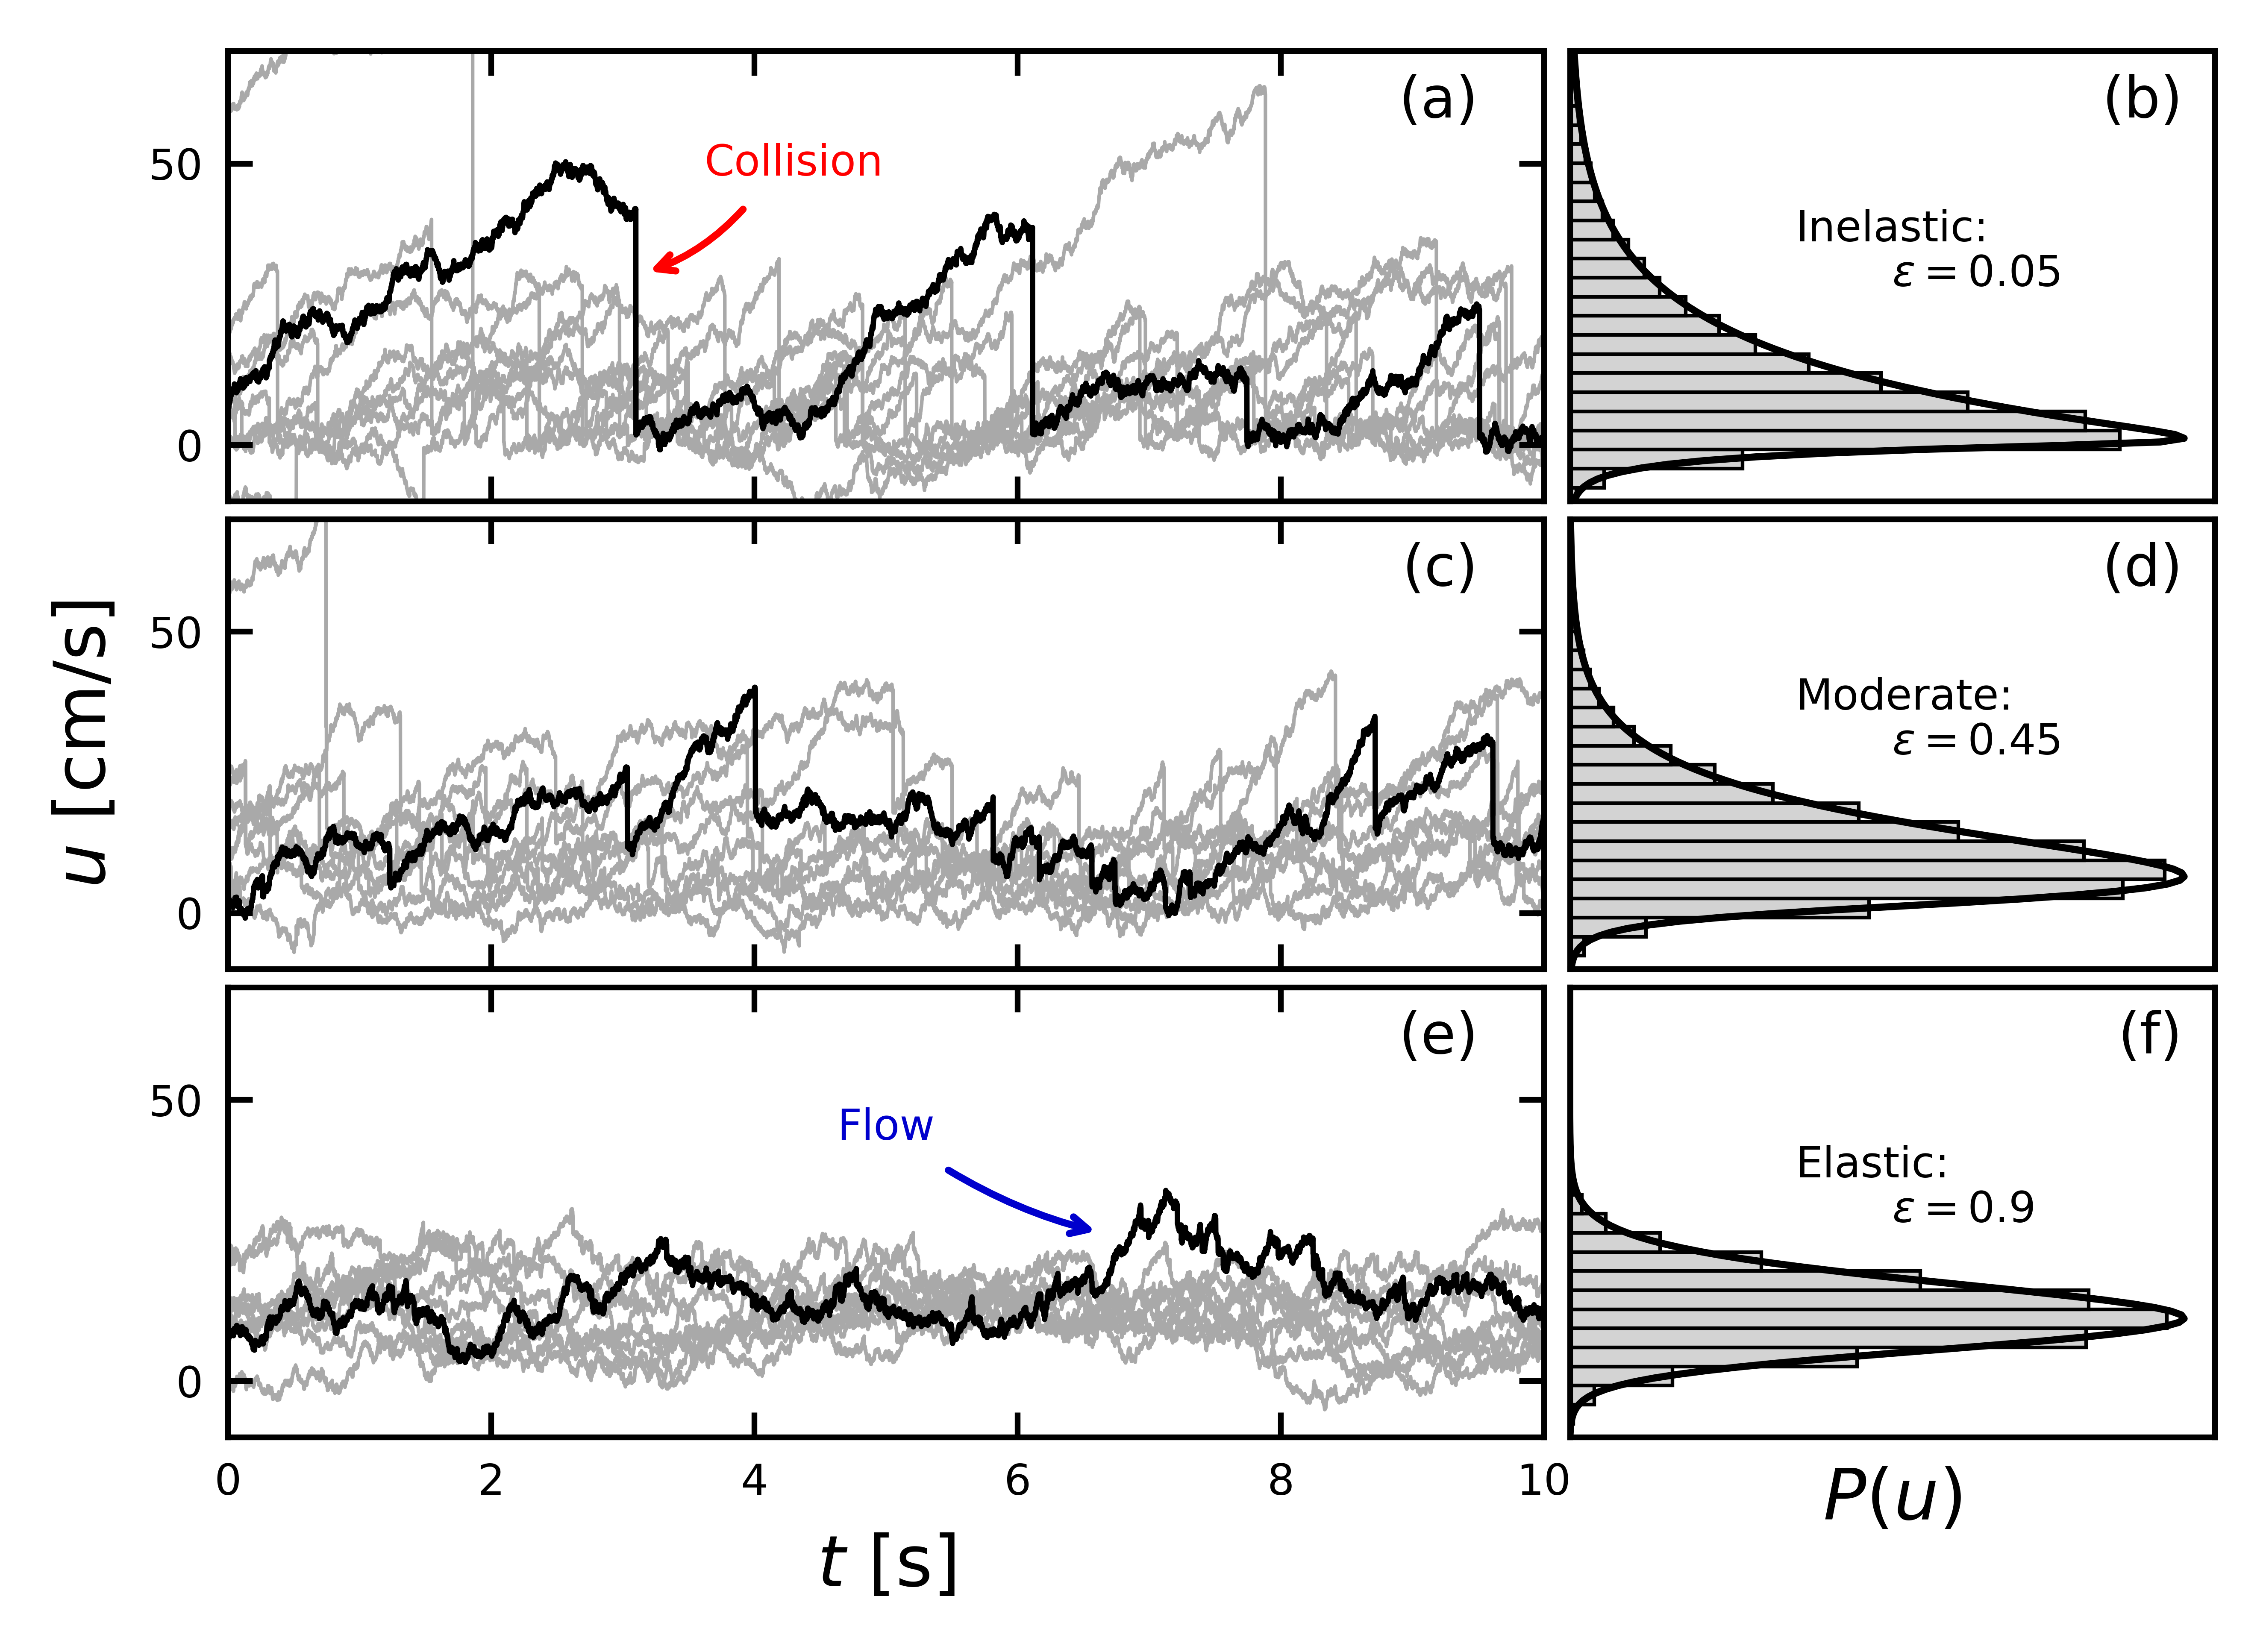
\includegraphics{./figures/ch5/Fig2pdfs.png}}
	\caption{Left and right panels are paired. Left panels show velocity realizations as gray traces. Velocities are calculated from Monte Carlo simulations. Individual realizations are singled out as black traces. Particle-bed collisions imply sudden downward-velocity jumps. Flow forces generate fluctuating positive accelerations between collisions. Right panels show simulated histograms of particle velocities and exact solutions from equation \ref{eq:steadystate}. As elasticity $\ve$ varies, the particle velocity distributions interpolate between exponential (inelastic) and Gaussian (elastic) forms.}
	\label{fig:fig2}
\end{figure}
This figure reveals an apparent transition from exponential-like to Gaussian-like velocity distributions as  collisions vary from more inelastic ($\ve \rightarrow 0$) to more elastic ($\ve \rightarrow 1$). In between, the full distribution \ref{eq:steadystate} resembles a Gamma distribution, although it is represented by equation \ref{eq:steadystate}, not a Gamma distribution.


\subsection{Exponential and Gaussian regimes: limits to earlier work}
\label{sec:langmodelcomparison}

In fact, the apparent transition from exponential to Gaussian in figure \ref{fig:fig2} can be demonstrated from equation \ref{eq:steadystate}. Despite its complex appearance, simple Gaussian and exponential forms derive from this equation as exact mathematical limits.
When particle-bed collisions are completely inelastic ($\ne = 0$), \ref{eq:steadystate} becomes an exponential distribution, and when they are completely elastic ($\nu = 1$), \ref{eq:steadystate} becomes Gaussian.
Figure \ref{fig:fig3} demonstrates in detail the approach of the distribution toward these limits.
\begin{figure}
	\centerline{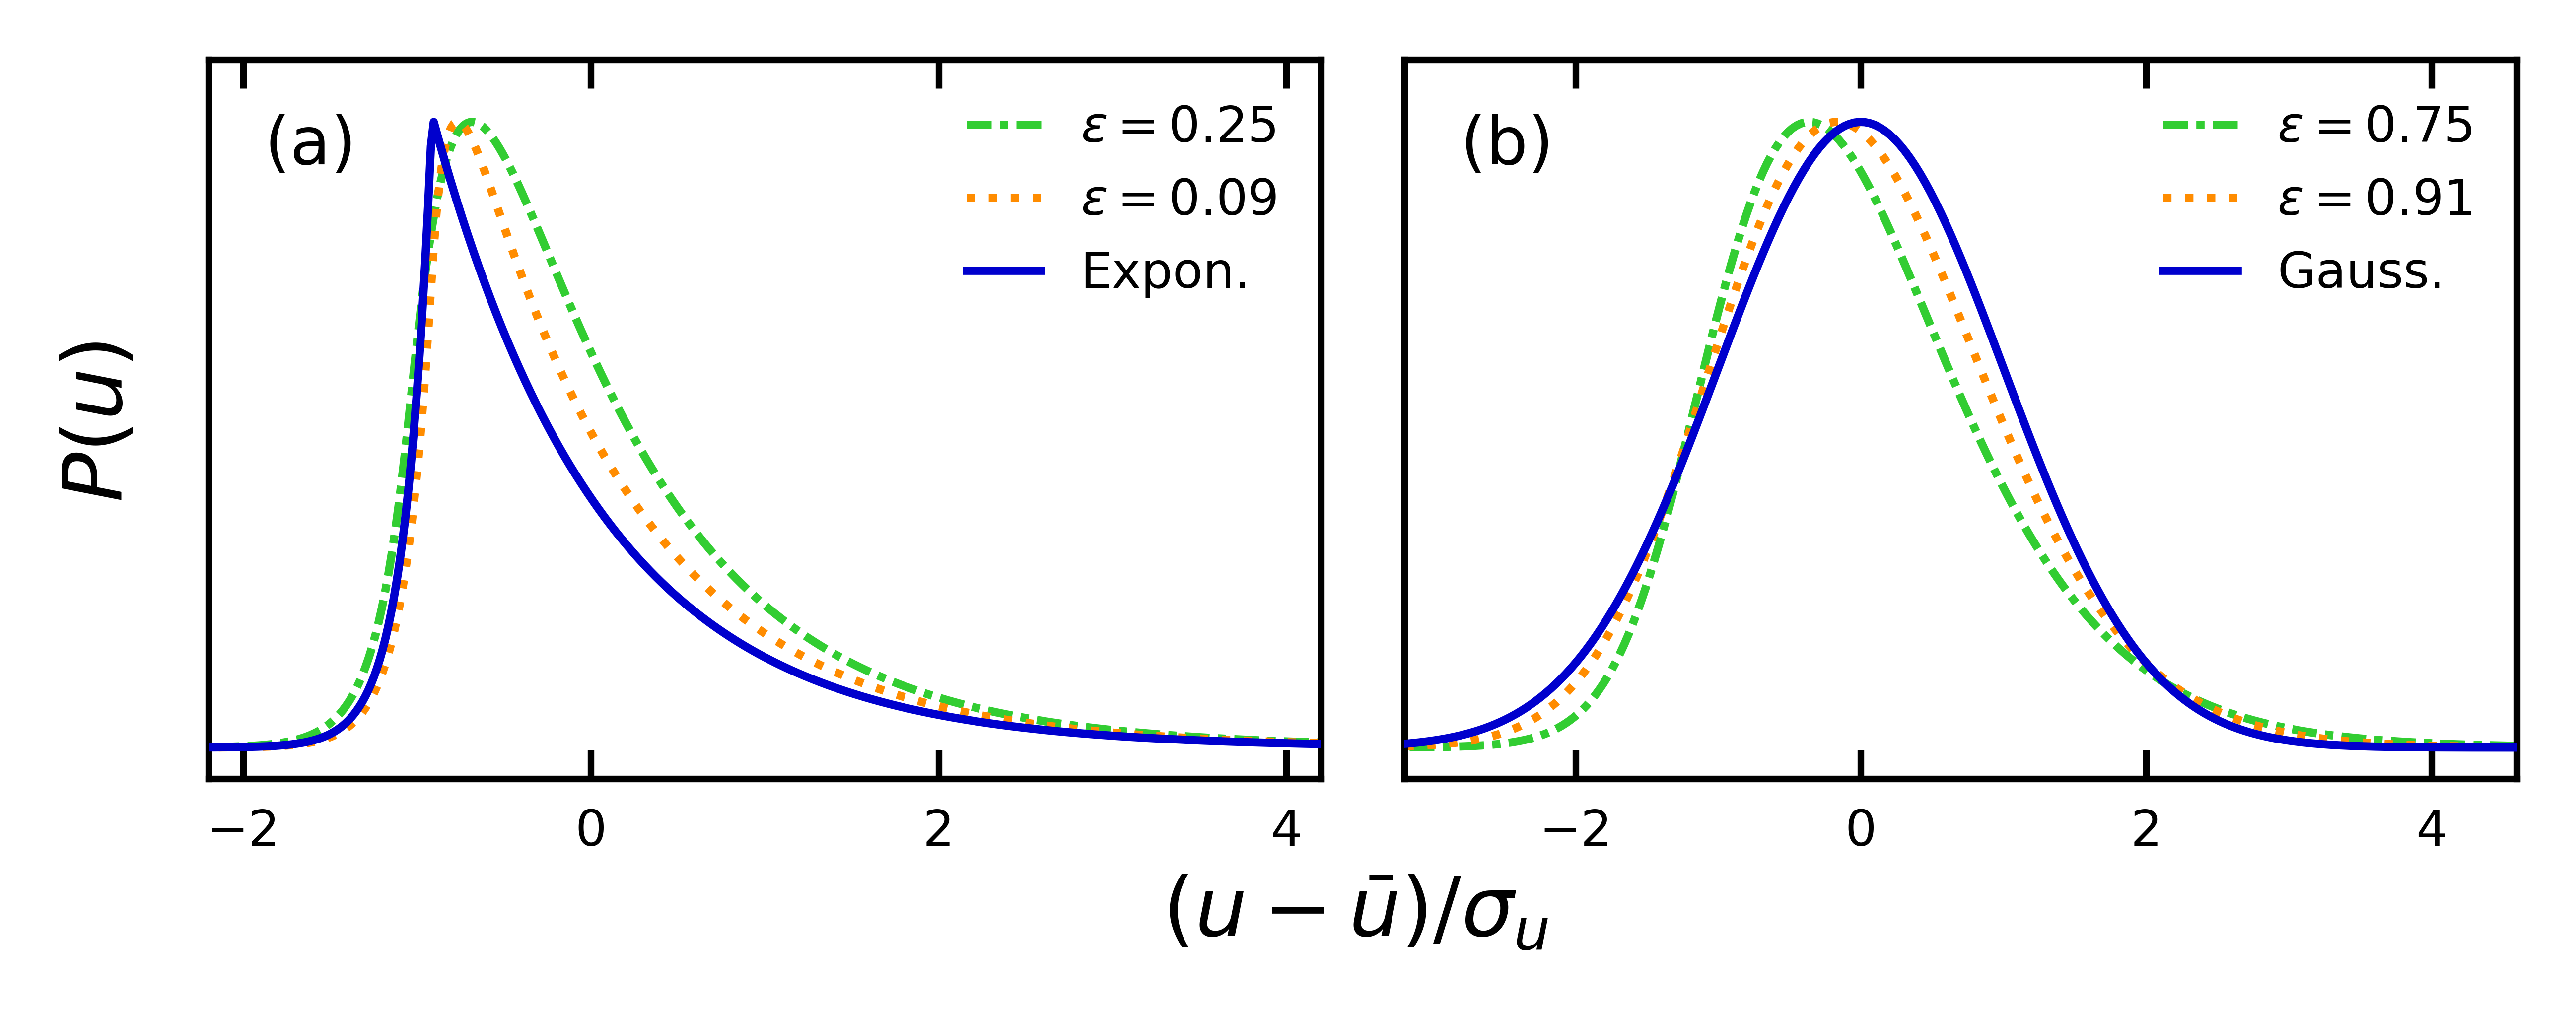
\includegraphics{./figures/ch5/Fig3asymptotic.png}}
	\caption{The particle velocity distribution approaches an exponential distribution in (a) as particle-bed collisions become extremely elastic ($\ve \rightarrow 1$), and it approaches a Gaussian in (b) as they become extremely inelastic ($\ve \rightarrow 0$). On the abscissa, the mean sediment velocity is standardized by its mean $\bar{u}$ and standard deviation $\sigma_u$. }
	\label{fig:fig3}
\end{figure}

The exponential limit of \ref{eq:steadystate} as $\ve \rightarrow 0$ is easy to see. Taking $\ve \rightarrow 0 $ in \ref{eq:steadystate}, all terms in the series except for that with $l=0$ become exponentially small, leaving behind the same two-sided exponential distribution derived by \cite{Fan2014} up to differences in notation:
\be P(u) = \frac{d}{\sqrt{\gamma^2 + 4d}}e^{\frac{\gamma u }{2 d} - \frac{\sqrt{\gamma^2 + 4 d}|u|}{2d}}. \ee
Thus, for bed load transport conditions with typically very inelastic particle-bed collisions, we can expect exponential-like velocities and large deviations from a Gaussian behavior.

The Gaussian limit as $\ve \rightarrow 1$ of \ref{eq:steadystate} is more difficult to evaluate. The challenge is that the statistical moments \ref{eq:mean} and \ref{eq:varu} diverge at the same time as the denominator factors of the distribution \ref{eq:steadystate}. In the appendix section \ref{sec:langextremes} I return instead to the original equation \ref{eq:governer} to evaluate the completely elastic limit, obtaining
\be P(u) = \frac{1}{\sqrt{2\pi\sigma_u^2}}e^{-\frac{(u-\bar{u})^2}{2\sigma_u^2}}. \label{eq:gaussian}\ee
This result is identical to the velocity distribution derived by \citet{Ancey2014}, up to notation.

\subsection{Comparison with experimental data}
\label{sec:langexperimentcomparison}

A variety of velocity distributions have been observed in bedload transport experiments, ranging from exponential to Gaussian in shape. 
This section compares these with the theoretical result eq. \ref{eq:steadystate}.
Comparing eq. \ref{eq:steadystate} with experimental data requires values for the steady component of the drag force $\Gamma$, the particle mass $m$, the magnitude of turbulent drag fluctuations $D$, the rate of particle-bed collisions $\nu$, and the mode elasticity of collisions $\varepsilon$.

This section compares eq. \ref{eq:steadystate} with the results of six different experiments.
In each case, the particle mass is computed from experimental parameters assuming spherical sediment as $m = \pi \rho_s d^3/6$, where $\rho_s$ is the sediment density and $d$ is the particle diameter. The steady component of the drag force is estimated as
\be \Gamma =  \frac{\pi}{8}\rho C_D(\Rey_p) d^2 u_\ast^2,\ee
where $\rho$ is the fluid density and $C_D(\Rey_p)$ is the drag coefficient, given as \citep{Clift1978,Gonzalez2017}
\be C_D = \frac{24}{\Rey_p}( 1 + 0.194 \Rey_p^{0.631}). \ee
Particle Reynolds numbers are estimated using the shear velocity: $\Rey_p= u_\ast d/nu$. 

The magnitude $D$ of turbulent fluctuations is eliminated with the mean and variance of the particle velocity. The remaining coefficients in the model, the dissipation per collision $\ve$ and the collision rate $\nu$, are treated as calibration parameters and are tuned to provide best fit between the distribution \ref{eq:steadystate} and the experimental data.

The parameters for each experiment and the best-fit calibration parameters are collated in table \ref{tab:calib}, while the results of fitting the model to the available experimental data are shown in figure \ref{fig:fig4ch5}.
\begin{table}
	\begin{center}
		\def~{\hphantom{0}}
		\begin{tabular}{l|ccccccc}
			Experiment & $d$ [$mm$] & $u_\ast$ [$cm/s$]  & $\Rey_p$ [-] & $\St$ [-] & $\Fro$ [-] & $\ve$ [-] & $\nu$ [$s^{-1}$] \\
			\toprule 
			\textit{(a) Fathel et al} & 0.5 & 2.0 & 9.97 & 2.9 & 0.3 & 0.08 & 24. \\ 
			\textit{(b) Lajeu. et al} & 2.2 & 4.4 & 99.  & 29.  	& 1.5 & 0.21 & 2.6 \\ 
			\textit{(c) Liu et al}    & 1.1 & 8.6 & 94.  & 29.  & 0.3 & 0.28 & 34.  \\ 
			\textit{(d) Heyman et al} & 6.4 & 9.7 & 620. & 180. & 1.3 & 0.96 & 13. \\ 
			\textit{(e) Ancey et al}  & 8.0 & 7.4 & 590. & 170. & 2.1 & 0.92 & 4.8 \\ 
			\textit{(f) Martin et al} & 7.1 & 5.8 & 410. & 120. & 3.7 & 0.89 & 2.1  \\ 
		\end{tabular}
		\caption{Parameters used to fit the distributions in figure \ref{fig:fig4ch5}. The first five columns involve data from the experiments for particle diameter $d$, shear velocity $u_\ast$, particle Reynolds number $\Rey_p$, Stokes number $\St$, and Froude number $\Fro$. The final two columns involve values that were tuned to fit the theoretical distribution \ref{eq:steadystate} to the experimental data, the dissipation $\ve$ and the collision rate $\nu$. Units are indicated in square brackets. One can see a generally increasing relationship between particle size and elasticity, and likewise a decreasing relationship between particle size and collision frequency. }
		\label{tab:calib}
	\end{center}
\end{table}
In every case, good agreement is obtained between the theoretical and empirical velocity disributions, suggesting that the Langevin model \ref{eq:langevin} captures the essential physics.
\begin{figure}
	\centerline{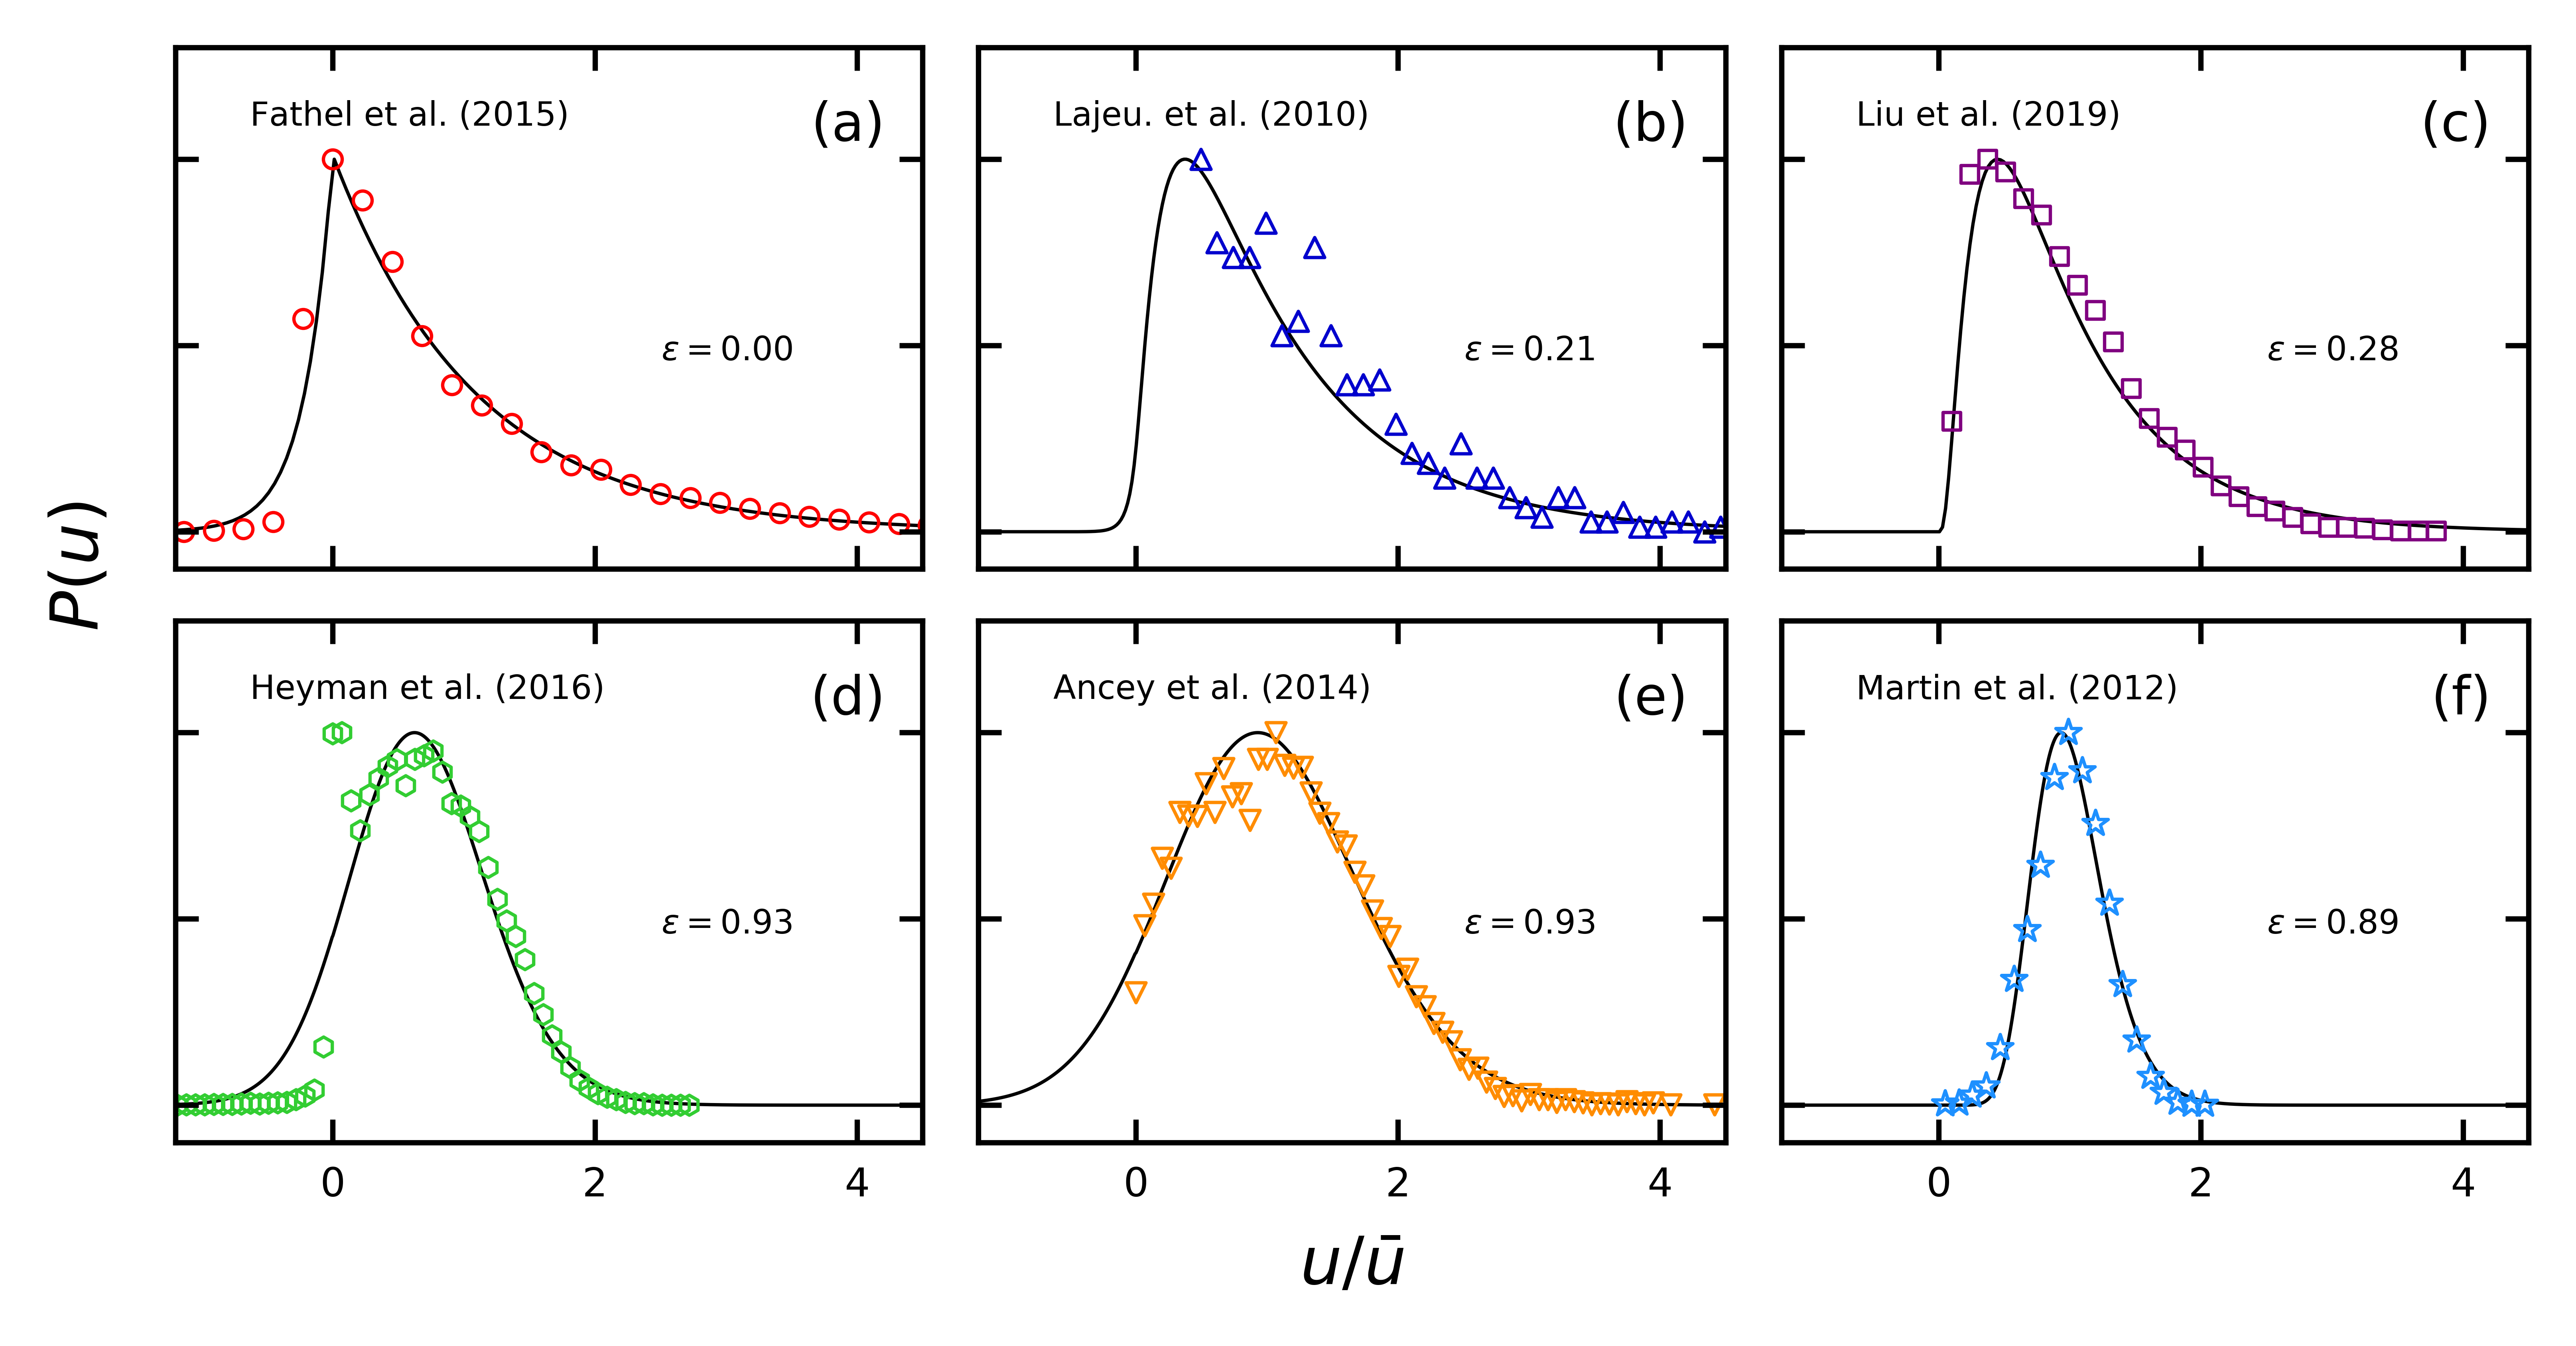
\includegraphics{./figures/ch5/Fig4expComparison.png}}
	\caption{This figure compares the available experimental data on velocity distributions and the theoretical velocity distribution \ref{eq:steadystate} with parameters $\nu$, $\varepsilon$, and $D$ treated as calibration parameters. In all cases there is good agreement, indicating that the model is capable of the range of distributions exhibited by the experimental data.} \label{fig:fig4ch5}
\end{figure}


\section{Discussion}
\label{sec:langdiscussion}

In this final chapter I developed a Langevin description of bed load sediment transport which includes episodic collisions between particles and the bed.
The model relates the shape of the instantaneous streamwise particle velocity distribution to the elasticity of particle-bed collisions.
This work generalizes earlier approaches available in the literature which did not treat episodic collisions \citep{Ancey2014,Fan2014}, and provides a new physical explanation for the different streamwise sediment velocity distributions resolved in experiments.

Although in reality, the turbulent forces on moving sediment particles vary in a complex spatio-temporal way, I have approximated the fluid forces on bed load particles as spatially uniform Gaussian white noise. Even though the non-Gaussian and history-dependent aspects of fluid turbulence certainly do impact sediment entrainment \citep{Cameron2020,Celik2014}, this flow model appears more or less justified since sediment transport experiments provide similar velocity distributions regardless of whether the flow is viscous or turbulent \citep{Lajeunesse2010, Charru2004}, and since particle relaxation times are typically long compared to the timescales of turbulent fluctuations \citep{Hofland2006,Schmeeckle2007,Nakagawa1981}.

The model developed in this chapter described particle-bed collision forces as a sequence of instantaneous impulses in an approach that is reminiscent of the kinetic theory of gases \citep{Landau1969}.
The effect of each collision on the streamwise particle velocities was described by a simple elasticity-like coefficient.
Although such approximate descriptions of particle-particle collisions are common in the theory of granular gases, the elasticity coefficient introduced here is not equivalent to the ``coefficient of restitution" typically applied in granular gas theory.
The coefficient of resitution is defined normal to the contact plane of two particles during a collision, and it characterizes energy loss due to deformation of the colliding particles in the absence of a viscous fluid \citep{Brach1992,Ismail2008}.

In bedload transport, colliding particles are submerged in a viscous fluid, and this introduces additional damping processes besides particle deformation \citep{Joseph2001,Yang2006,Schmeeckle2001}.
The model developed here did not consider these viscous forces, nor did it explicitly model the geometry of collisions, as $\ve$ was defined as a parameter applying to the downstream velocity only.
Thus, although I have included episodic particle-bed collisions in a stochastic sediment transport model for the first time, the key parameter ($\ve$) in this formulation has a rather heuristic character and is not clearly related to the coefficient of restitution from granular gas theory.
Future studies should formulate particle-bed collisions in stochastic sediment transport models considering more details of collision geometry \citep{Sekine1992}, fluid-particle interactions \citep{Marshall2011}, and traditional restitution \citep{Brach1989} using the present study as a starting point. 

\subsection{Does the velocity distribution depend on particle size?}

Several researchers have considered why particle velocity distributions differ from one experiment to the next.
One prevailing view is that it relates to flow hydraulics \citep{Wu2020}. Many of the experiments producing Gaussian velocity distributions were conducted in supercritical flows \citep[e.g.][]{Heyman2016,Martin2012,Ancey2014}, whereas many producing exponential distributions were conducted in subcritical flows \citep[e.g.][]{Fathel2015,Charru2004,Seizilles2014}.
However several experiments run counter to this hypothesis.
The experiments of \citet{Lajeunesse2010} produced distinctly exponential velocity distributions in flows well within the supercritical regime ($\Fro=1.5$), whereas \citet{Liu2019} produced Gamma-like distributions in the subcritical regime ($\Fro=0.3$).

An alternative viewpoint, formulated in this chapter, is that the shape of the velocity distribution originates from granular interactions.
Particle size enters the Langevin model \ref{eq:langevin} explicitly within the steady component of the drag, but it may also enter implicitly through the elasticity parameter $\ve$.
The analytical velocity distribution \ref{eq:steadystate} was fit to six different experimental datasets in figure \ref{fig:fig4ch5}, and the best fit parameters required to for these fits were presented in table \ref{tab:calib}.
These fit parameters suggest collisions are generally less elastic for smaller particle sizes, whereas they are more elastic for larger particle sizes. This suggests that the amount of momentum dissipated by collisions may depend on particle size.

Because the elasticity $\ve$ lumps together collision geometry and dissipation effects, it is challenging to attribute the increasing relationship between elasticity and particle size evident in table \ref{tab:calib} directly to particle size.
Yet this would be consistent with experiments of idealized particle collisions in viscous fluids. These demonstrate that momentum dissipation varies sharply with particle size, being more elastic for large particles, and less elastic for small particles \citep{Joseph2001,Yang2006,Schmeeckle2001}, exactly like the trend in the table.
A definite conclusion that particle size controls the shape of the bedload velocity distribution requires additional experimental and theoretical study. This chapter nevertheless produces suggestive ideas.

\section{Summary}
\label{sec:langconclusion}
This chapter has presented a Langevin description of individual bedload particles saltating downstream through episodic collisions.
The model suggests that episodic particle-bed collisions control the shape of the particle velocity distribution, and it is the first model to describe the full range of bedload velocity distributions that have been reported in experimental studies.

This work hints that particle size, and not flow hydraulics, may be primarily responsible for the different bedload velocity distributions obtained in experiments, although future study is required for a definite conclusion.
The next step is to build up the episodic collision model presented in this chapter to include the geometric details of particle-bed collisions.
Such an effort would produce additional insight into the controls of transverse, vertical, and rotational movements on the downstream velocities of individual grains.

